%! Author = Juniell
%! Date = 07.05.2021

% Preamble
\documentclass[a4paper, 14pt]{extarticle}

% Packages
\usepackage[T2A]{fontenc}
\usepackage{natbib}
\usepackage{graphicx}
\usepackage[english, russian]{babel}
\usepackage{fontspec}
\usepackage{amsmath}
\usepackage{amsfonts}
\usepackage{amssymb}
\usepackage{amsthm}
\usepackage{mathtools}
\usepackage{mathrsfs}
\usepackage{fullpage}
\usepackage{ulem}
\usepackage{setspace}
\usepackage{listings}
\usepackage{indentfirst}
\usepackage[left=2cm,right=1.5cm,top=2cm,bottom=2cm]{geometry}
\usepackage{xcolor}
\usepackage{float}
\usepackage{csquotes}
\usepackage{hyperref}
\usepackage{graphics}

\definecolor{urlcolor}{HTML}{0000FF} % цвет ссылок
\definecolor{linkcolor}{HTML}{000000} % цвет гиперссылок
\hypersetup{pdfstartview=FitH, linkcolor=linkcolor, urlcolor=urlcolor, colorlinks=true}

\setmainfont{Times New Roman}
\setlength{\parindent}{5ex}
\setlength{\parskip}{1em}
\renewcommand{\baselinestretch}{1}

\graphicspath{{resources/Images}}

\definecolor{buzzlightyear}{HTML}{8757A5}
\definecolor{grass}{HTML}{738D06}
\definecolor{literal}{HTML}{F18A2B}
\definecolor{commentcolor}{HTML}{8E908B}

\lstdefinestyle{habrstyle}{
    backgroundcolor=\color{white},
    commentstyle=\color{commentcolor},
    keywordstyle=\bfseries\color{buzzlightyear},
    numberstyle=\tiny\color{commentcolor},
    stringstyle=\color{grass},
    basicstyle=\ttfamily\footnotesize,
    breakatwhitespace=false,
    breaklines=true,
    captionpos=b,
    keepspaces=true,
    numbers=left,
    numbersep=5pt,
    showspaces=false,
    showstringspaces=false,
    showtabs=false,
    tabsize=4,
    language=Python
}

\lstset{style=habrstyle}


% Document
\begin{document}
% Титульный лист
    \begin{center}
        \begin{center}
            \hfill \break
            \normalsize{Санкт-Петербургский государственный политехнический}\\
            \normalsize{университет Петра Великого}\\
            \hfill \break
            \normalsize{\textbf{Высшая школа интеллектуальных систем и}}\\
            \normalsize{\textbf{суперкомпьютерных технологий}}\\
            \hfill \break
            \hfill \break
            \hfill \break
            \hfill \break
            \hfill \break
            \normalsize{Отчёт по лабораторной работе №4}\\
            \normalsize{Дисциплина: Телекоммуникационные технологии}\\
            \normalsize{Тема: Шум}\\
        \end{center}
        \hfill \break
        \hfill \break
        \hfill \break
        \hfill \break
        \hfill \break
        \hfill \break
        \hfill \break
        \hfill \break
        \hfill \break
        \hfill \break
        \begin{tabbing}
            Выполнил студент гр. 3530901/80201 \`В.А. Пучкина\\
            \\
            Преподаватель: \`Н.В. Богач\\
        \end{tabbing}
        \hfill \break
        \hfill \break
        \hfill \break
        \hfill \break
        \begin{center}
            Санкт-Петербург\\
            2021
        \end{center}
        \thispagestyle{empty}
    \end{center}

% Оглавление
    \newpage
    \tableofcontents

% Список иллюстраций
    \newpage
    \listoffigures

% Список листингов
    \newpage
    \lstlistoflistings

% ---------------------------------------------- Упражнение 4.1 ----------------------------------------------
    \newpage
    \section{Упражнение 4.1}
    \label{sec:task1}

    Это упражнение направлено на знакомство с шумом. А потому необходимо скачать записи некоторых природных источников
    шума и вычислить спектры каждого из них.

    \subsection{Шум моря}
    \label{subsec:task1_sea}

    Для начала была скачена \href{https://freesound.org/people/Soarer/sounds/13793/}{эта} запись шума морских волн.
    Теперь необходимо считать скаченный файл и получить \texttt{wave}. Тут же прослушаем запись.

    \begin{lstlisting}[caption= Чтение скаченного файла., label={lst:task1_read_sea}]
sea_wave = read_wave('resources/Sounds/task1_north_sea.wav')
sea_wave.make_audio()   \end{lstlisting}

    Теперь выберем походящий сегмент и получим его линейный спектр.

    \begin{lstlisting}[caption= Выбор сегмента и получение его линейного спектра., label={lst:task1_sea_spectrum_lin}]
sea_segment = sea_wave.segment(start=3, duration=1)
sea_spectrum = sea_segment.make_spectrum()
sea_spectrum.plot_power()
decorate(ylabel='Power', xlabel='Frequency (Hz)')
sea_segment.make_audio()    \end{lstlisting}

    \begin{figure}[h]
        \centering
        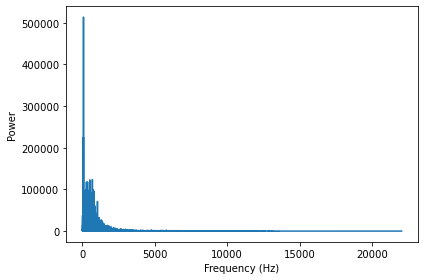
\includegraphics[width=0.8\linewidth]{resources/Images/task1_sea_spectrum_lin}
        \caption{Линейный спектр шума моря.}
        \label{fig:task1_sea_spectrum_lin}  \end{figure}

    Получим логарифмический спектр этого сегмента.

    \begin{lstlisting}[caption= Получение логарифмического спектра., label={lst:task1_sea_spectrum_log}]
sea_spectrum.plot_power()
decorate(ylabel='Power', xlabel='Frequency (Hz)', xscale='log', yscale='log')   \end{lstlisting}

    \begin{figure}[h]
        \centering
        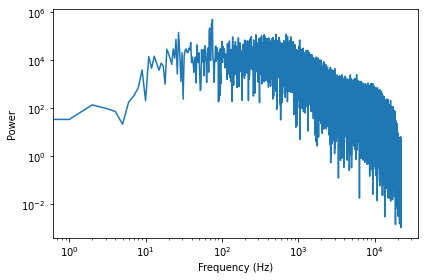
\includegraphics[width=0.8\linewidth]{resources/Images/task1_sea_spectrum_log}
        \caption{Логарифмический спектр шума моря.}
        \label{fig:task1_sea_spectrum_log}
    \end{figure}

    По полученным спектрам можно отнести этот шум к розовому или красному шуму (не к белому, потому что у нашего сигнала
    с увеличением частоты падает мощность). Однако отнести этот шум к какому-либо конкретному типу сложно.
    Также по логарифмическому спектру (Рис.\ref{fig:task1_sea_spectrum_log}) видно, что мощность сначала увеличивается,
    а потом уменьшается. Это обычное поведение для естественных источников шума.

    Также получим спектрограмму этого сегмента.

    \begin{lstlisting}[caption= Получение спектрограммы сегмента., label={lst:task1_sea_spectrum_log}]
sea_segment.make_spectrogram(256).plot(5000)
decorate(xlabel='Time (s)', ylabel='Frequency (Hz)')    \end{lstlisting}

    Теперь давайте посмотрим, как спектр изменяется во времени. Для этого выберем другой сегмент и сравним спектры второго
    сегмента с первым.

    \begin{lstlisting}[caption= Сравнение линейных спектров двух сегментов., label={lst:task1_sea_spectrum_lin_compare}]
sea_segment2 = sea_wave.segment(start=5, duration=1)
sea_spectrum2 = sea_segment2.make_spectrum()
sea_spectrum2.plot_power(color='red', alpha=0.5)
sea_spectrum.plot_power(color='blue', alpha=0.5)
decorate(ylabel='Power', xlabel='Frequency (Hz)')
sea_segment2.make_audio()   \end{lstlisting}

    \begin{figure}[H]
        \centering
        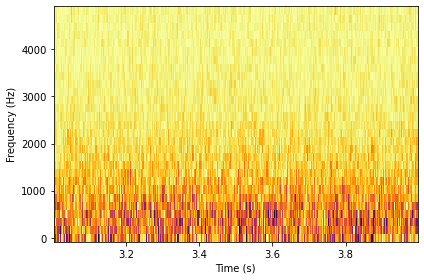
\includegraphics[width=0.8\linewidth]{resources/Images/task1_sea_spectrogram}
        \caption{Спектрограмма шума моря.}
        \label{fig:task1_sea_spectrogram}
    \end{figure}

    \begin{figure}[H]
        \centering
        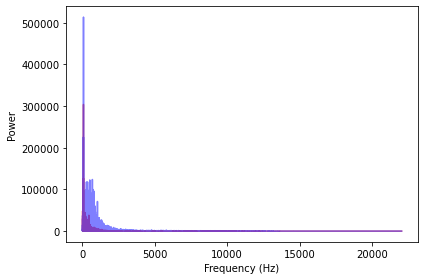
\includegraphics[width=0.8\linewidth]{resources/Images/task1_sea_spectrum_lin_compare}
        \caption{Сравнение линейных спектров первого (синий) и второго (красный) сегментов.}
        \label{fig:task1_sea_spectrum_lin_compare}
    \end{figure}

    И сравним логарифмические спектры.

    \begin{lstlisting}[caption= Сравнение логарифмических спектров двух сегментов., label={lst:task1_sea_spectrum_log_compare}]
sea_spectrum.plot_power(color='blue', alpha=0.5)
sea_spectrum2.plot_power(color='red', alpha=0.5)
decorate(ylabel='Power', xlabel='Frequency (Hz)', xscale='log', yscale='log')   \end{lstlisting}

    \begin{figure}[H]
        \centering
        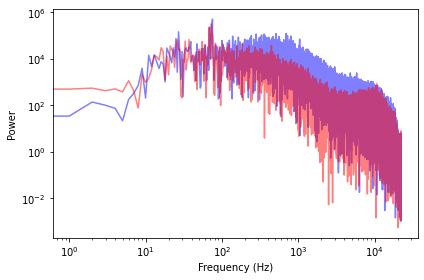
\includegraphics[width=0.8\linewidth]{resources/Images/task1_sea_spectrum_log_compare}
        \caption{Сравнение логарифмических спектров первого (синий) и второго (красный) сегментов.}
        \label{fig:task1_sea_spectrum_log_compare}
    \end{figure}

    Из полученных спектров (Рис.\ref{fig:task1_sea_spectrum_lin_compare} и Рис.\ref{fig:task1_sea_spectrum_log_compare})
    можно сделать вывод, что спектр шума моря с течением времени не изменяется.

    \newpage
    \subsection{Шум костра}
    \label{subsec:task1_fire}

    Теперь изучим запись шума костра, скаченную \href{https://freesound.org/people/inchadney/sounds/83986/}{отсюда}.
    Считаем файл, выберем походящий сегмент и получим его линейный спектр.

    \begin{lstlisting}[caption= {Чтение файла, выбор сегмента и получение линейного спектра.}, label={lst:task1_fire_spectrum_lin}]
fire_wave = read_wave('resources/Sounds/task1_fireplace.wav')
fire_segment = fire_wave.segment(start=12, duration=1)
fire_spectrum = fire_segment.make_spectrum()
fire_spectrum.plot_power()
decorate(ylabel='Power', xlabel='Frequency (Hz)')
fire_segment.make_audio()  \end{lstlisting}

    \begin{figure}[h]
        \centering
        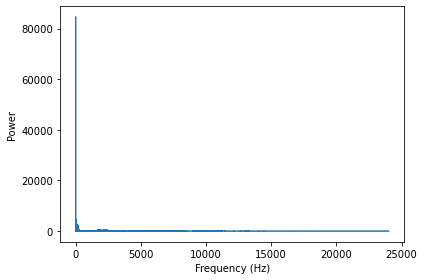
\includegraphics[width=0.8\linewidth]{resources/Images/task1_fire_spectrum_lin}
        \caption{Линейный спектр шума костра.}
        \label{fig:task1_fire_spectrum_lin}
    \end{figure}

    Получим логарифмический спектр выбранного сегмента.

    \begin{lstlisting}[caption= Получение логарифмического спектра., label={lst:task1_fire_spectrum_log}]
fire_spectrum.plot_power()
decorate(ylabel='Power', xlabel='Frequency (Hz)', xscale='log', yscale='log')   \end{lstlisting}

    По полученным спектрам шум костра так же, как и шум моря, можно отнести к розовому или красному шуму.
    Получим спектрограмму нашего сегмента.

    \begin{lstlisting}[caption= Получение спектрограммы сегмента., label={lst:task1_fire_spectrogram}]
fire_spectrum.plot_power()
decorate(ylabel='Power', xlabel='Frequency (Hz)', xscale='log', yscale='log')   \end{lstlisting}

    \begin{figure}[H]
        \centering
        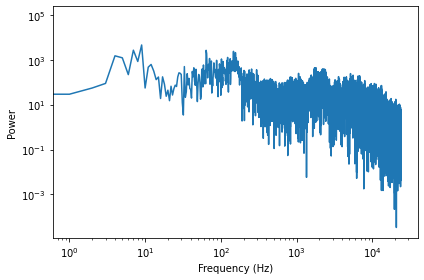
\includegraphics[width=0.7\linewidth]{resources/Images/task1_fire_spectrum_log}
        \caption{Логарифмический спектр шума костра.}
        \label{fig:task1_fire_spectrum_log}
    \end{figure}

    \begin{figure}[h]
        \centering
        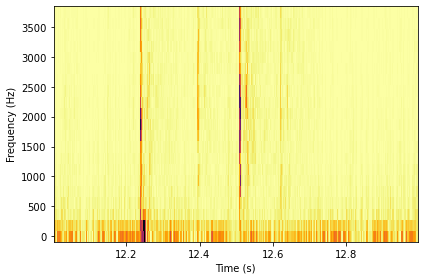
\includegraphics[width=0.7\linewidth]{resources/Images/task1_fire_spectrogram}
        \caption{Спектрограмма шума костра.}
        \label{fig:task1_fire_spectrogram}
    \end{figure}

    Теперь посмотрим, как спектр изменяется во времени. Для этого выберем другой сегмент и сравним линейные спектры второго
    сегмента с первым.

    \begin{lstlisting}[caption= Сравнение линейных спектров двух сегментов., label={lst:task1_fire_spectrum_lin_compare}]
fire_segment2 = fire_wave.segment(start=27, duration=1)
fire_spectrum2 = fire_segment2.make_spectrum()
fire_spectrum2.plot_power(color='red', alpha=0.5)
fire_spectrum.plot_power(color='blue', alpha=0.5)
decorate(ylabel='Power', xlabel='Frequency (Hz)')
fire_segment2.make_audio()
    \end{lstlisting}

    \begin{figure}[h]
        \centering
        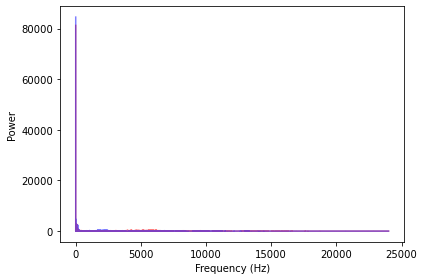
\includegraphics[width=0.8\linewidth]{resources/Images/task1_fire_spectrum_lin_compare}
        \caption{Сравнение линейных спектров первого (синий) и второго (красный) сегментов.}
        \label{fig:task1_fire_spectrum_lin_compare}
    \end{figure}

    Сравним также логарифмические спектры.

    \begin{lstlisting}[caption= Сравнение логарифмических спектров двух сегментов., label={lst:task1_fire_spectrum_log_compare}]
fire_spectrum.plot_power(color='blue', alpha=0.5)
fire_spectrum2.plot_power(color='red', alpha=0.5)
decorate(ylabel='Power', xlabel='Frequency (Hz)', xscale='log', yscale='log')   \end{lstlisting}

    \begin{figure}[H]
        \centering
        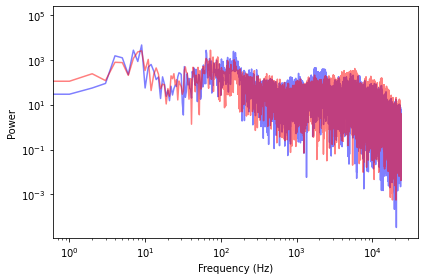
\includegraphics[width=0.8\linewidth]{resources/Images/task1_fire_spectrum_log_compare}
        \caption{Сравнение логарифмических спектров первого (синий) и второго (красный) сегментов.}
        \label{fig:task1_fire_spectrum_log_compare}
    \end{figure}

    Из полученных спектров (Рис.\ref{fig:task1_fire_spectrum_lin_compare} и Рис.\ref{fig:task1_fire_spectrum_log_compare})
    можно сделать вывод, что спектр шума костра с течением времени не изменяется.

    В ходе выполнения данного упражнения были проанализированы линейные и логарифмические спектры шума моря и костра.
    Также были рассмотрены их спектрограммы и проанализировано изменение их спектров в течение времени.
    Был сделан вывод, что спектры этих шумов с течением времени не изменяются.

    \newpage

% ---------------------------------------------- Упражнение 4.2 ----------------------------------------------
    \section{Упражнение 4.2}
    \label{sec:task2}

    В данном упражнении необходимо реализовать метод Бартлетта и использовать его для оценки спектра мощности шумового
    сигнала.

    Итак, начнём с реализации метода Бартлетта.

    \begin{lstlisting}[caption= Метод Бартлетта., label={lst:task2_bartlett}]
def bartlett (wave, seg_length=512, win_flag=True):
    spectrogram = wave.make_spectrogram(seg_length, win_flag)
    spectrums = spectrogram.spec_map.values()
    psds = [spectrum.power for spectrum in spectrums]
    hs = numpy.sqrt(sum(psds) / len(psds))
    fs = next(iter(spectrums)).fs
    spectrum = Spectrum(hs, fs, wave.framerate)
    return spectrum \end{lstlisting}

    Теперь используем наш метод для оценки спектра мощности шумового сигнала. В качестве шумового сигнала возьмём шум
    моря из \S\,\ref{subsec:task1_sea}.

    \begin{lstlisting}[caption= Оценка спектра мощности двух сегментов., label={lst:task2_spectrum}]
bartlett(sea_segment).plot_power(color='blue')
bartlett(sea_segment2).plot_power(color='red')
decorate(ylabel='Power', xlabel='Frequency (Hz)', xscale='log', yscale='log')   \end{lstlisting}

    \begin{figure}[h]
        \centering
        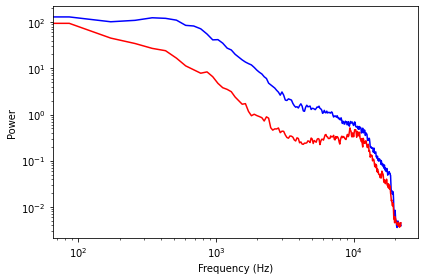
\includegraphics[width=0.6\linewidth]{resources/Images/task2_spectrum}
        \caption{Сравнение спектров мощности двух сегментов.}
        \label{fig:task2_spectrum}
    \end{figure}

    Из Рис.\ref{fig:task2_spectrum} видно, что мощность и частота связаны. Конечно, они имеют не линейную, а более
    сложную связь, однако для разных сегментов эта связь одинакова.

    В ходе данного упражнения был реализован метод Бартлетта, после чего с его помощью была проведена оценка спектра
    мощности шума моря. Был сделан вывод, что мощность и частота имеют сложную связь, однако для разных сегментов эта
    связь одинакова.

    \newpage

% ---------------------------------------------- Упражнение 4.3 ----------------------------------------------
    \section{Упражнение 4.3}
    \label{sec:task3}

    В этом упражнении необходимо провести следующий эксперимент: скачать с \href{https://www.coindesk.com/price/bitcoin}{этого сайта}
    исторические данные о ежедневной цене BitCoin в виде CSV-файла, затем вычислить спектр цен BitCoin и оценить, на
    какой вид шума похож полученный спектр.

    Итак, скачаем курс BTC/USD за всё время с указанного выше сайта, считаем и преобразуем его в \texttt{wave}.

    \begin{lstlisting}[caption= Перобразование файла с курсом BitCoin в \texttt{wave}., label={lst:task3_wave_btc}]
import pandas

df = pandas.read_csv('resources/task3_BTC_USD_2013-10-01_2021-05-07.csv', parse_dates=[0])
ys = df['Closing Price (USD)']
ts = df.index

wave_btc = Wave(ys, ts, framerate=1)
wave_btc.plot()
decorate(xlabel='Time (days)')  \end{lstlisting}

    \begin{figure}[h]
        \centering
        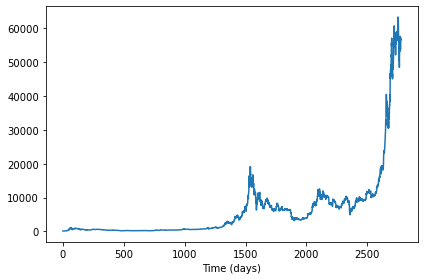
\includegraphics[width=0.7\linewidth]{resources/Images/task3_wave_btc}
        \caption{Курс BitCoin.}
        \label{fig:task3_wave_btc}
    \end{figure}

    Теперь получим спектр курса BitCoin и его значение его наклона.

    \begin{lstlisting}[caption= Получение спектра и наклона курса BtCoin., label={lst:task3_spectrum_btc}]
spectrum_btc = wave_btc.make_spectrum()
spectrum_btc.plot_power()
decorate(xlabel='Frequency (1/days)', xscale='log', yscale='log')
spectrum_btc.estimate_slope()[0]    \end{lstlisting}

    \begin{figure}[h]
        \centering
        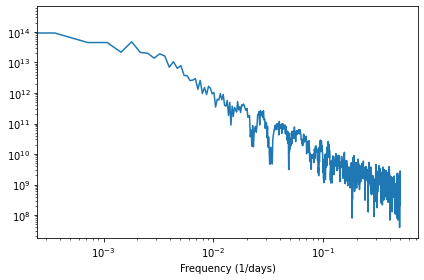
\includegraphics[width=0.8\linewidth]{resources/Images/task3_spectrum_btc}
        \caption{Спектр курса BitCoin.}
        \label{fig:task3_spectrum_btc}
    \end{figure}

    Полученный спектр (Рис.\ref{fig:task3_spectrum_btc}) напоминает спектры розового или красного шумов.
    Кроме того, наклон получился равным -1.803467606343994, что можно округлить до -1,8. Красный шум имеет наклон -2,
    а потому курс BitCoin это либо красный, либо розовый шум.

    В ходе данного упражнения был проведён интересный эксперимент с BitCoin. Был скачан курс BTC/USD за всё время,
    после чего получен его \texttt{wave} и спектр. По полученным результатам был сделан вывод, что курс BTC/USD сложно
    отнести к конкретному виду шума, так как он похож и на красный, и на розовый шумы.

    \newpage

% ---------------------------------------------- Упражнение 4.4 ----------------------------------------------
    \section{Упражнение 4.4}
    \label{sec:task4}

    В этом упражнении необходимо написать класс \texttt{UncorrelatedPoissonNoise}, наследующий \texttt{thinkdsp.\_Noise}
    и имеющий \texttt{evaluate}. Для генерации случайных величин из распределения Пуассона следует использовать
    \texttt{Np.random.poisson}. Затем с помощью этого класса необходимо сгенерировать и прослушать сигнал в несколько
    секунд, после чего вычислить его спектр мощности.

    Итак, начнём с написания класса \texttt{UncorrelatedPoissonNoise}.

    \begin{lstlisting}[caption= Класс \texttt{UncorrelatedPoissonNoise}., label={lst:task4_class}]
class UncorrelatedPoissonNoise(Noise):
    def evaluate(self, ts):
         ys = numpy.random.poisson(self.amp, len(ts))
         return ys  \end{lstlisting}

    \subsection{Сигнал с amp = 0.001}
    \label{subsec:task4_small}

    Теперь с помощью этого класса сгенерируем сигнал (\texttt{amp = 0.001}), получим его \texttt{wave} и прослушаем его.

    \begin{lstlisting}[caption= Генерация сигнала с \texttt{amp = 0.001}., label={lst:task4_small_signal}]
poisson_signal = UncorrelatedPoissonNoise(amp=0.001)
poisson_wave = poisson_signal.make_wave(duration=1, framerate=10000)
poisson_wave.plot()
poisson_wave.make_audio()   \end{lstlisting}

    Полученный звук действительно напоминает <<щелчки>> счётчика Гейгера. Вычислим ожидаемое и реальное количество
    <<щелчков>>.

    \begin{lstlisting}[caption= Проверка количества частиц \texttt{(amp = 0.001)}., label={lst:task4_small_check}]
expected = 0.001 * 10000 * 1
actual = sum(poisson_wave.ys)
print('expected = ', expected, '\nactual = ', actual)\end{lstlisting}

    \begin{figure}[H]
        \centering
        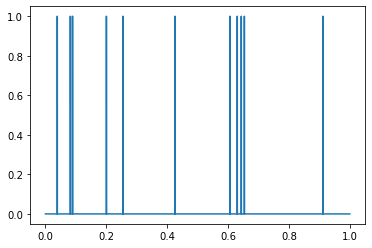
\includegraphics[width=0.8\linewidth]{resources/Images/task4_small_wave}
        \caption{\texttt{Wave} сгенерированного сигнала (\texttt{amp = 0.001}).}
        \label{fig:task4_small_wave}
    \end{figure}

    Был получен следующий результат: expected = 10.0, actual = 11. Эти значения близки, а потому всё верно.
    Также можно заметить, что количество фактических <<щелчков>> совпадает с количеством пиков на Рис.\ref{fig:task4_small_wave}.

    Теперь получим логарифмический спектр сигнала.

    \begin{lstlisting}[caption= Вычисление логарифмического спектра сигнала \texttt{(amp = 0.001)}., label={lst:task4_small_spectrum_log}]
poisson_spectrum = poisson_wave.make_spectrum()
poisson_spectrum.plot_power()
decorate(ylabel='Power', xlabel='Frequency (Hz)', xscale='log', yscale='log')   \end{lstlisting}

    Как можно видеть из Рис.\ref{fig:task4_small_spectrum_log}, спектр сгенерированного сигнала напоминает спектр белого
    шума. Чтобы в этом убедиться, оценим его наклон.

    \begin{lstlisting}[caption= Вычисление наклона \texttt{(amp = 0.001)}., label={lst:task4_small_slope}]
poisson_spectrum.estimate_slope().slope \end{lstlisting}

    \begin{figure}[H]
        \centering
        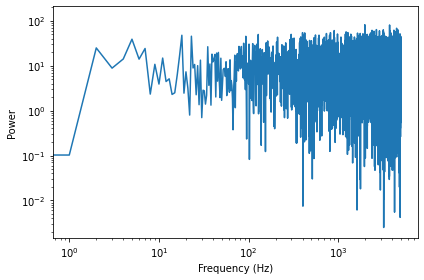
\includegraphics[width=0.8\linewidth]{resources/Images/task4_small_spectrum_log}
        \caption{Логарифмический спектр сгенерированного сигнала (\texttt{amp = 0.001}).}
        \label{fig:task4_small_spectrum_log}
    \end{figure}

    Было получено значение 0.006434726137836779, что близко к 0. А это как раз характерно для белого шума.

    \newpage
    \subsection{Сигнал с amp = 1}
    \label{subsec:task4_large}

    Теперь сгенерируем сигнал с большим значением \texttt{amp}. И проделаем для него то же самое.

    \begin{lstlisting}[caption= Генерация сигнала с \texttt{amp = 1}., label={lst:task4_large_signal}]
poisson_signal = UncorrelatedPoissonNoise(amp=1)
poisson_wave = poisson_signal.make_wave(duration=1, framerate=10000)
poisson_wave.plot()
poisson_wave.make_audio()   \end{lstlisting}

    \begin{figure}[h]
        \centering
        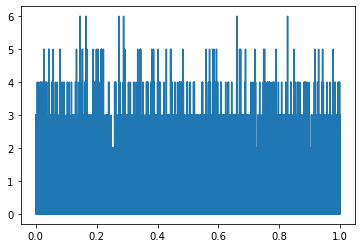
\includegraphics[width=0.7\linewidth]{resources/Images/task4_large_wave}
        \caption{\texttt{Wave} сгенерированного сигнала (\texttt{amp = 1}).}
        \label{fig:task4_large_wave}
    \end{figure}

    Этот звук уже напоминает белый шум. Вычислим ожидаемое и реальное количество <<щелчков>>.

    \begin{lstlisting}[caption= Проверка количества частиц \texttt{(amp = 1)}., label={lst:task4_large_check}]
expected = 1 * 10000 * 1
actual = sum(poisson_wave.ys)
print('expected = ', expected, '\nactual = ', actual)   \end{lstlisting}

    Был получен следующий результат: expected = 10000, actual = 10069. Эти значения близки, а потому всё верно.

    Получим логарифмический спектр сигнала.

    \begin{lstlisting}[caption= Вычисление логарифмического спектра сигнала \texttt{(amp = 1)}., label={lst:task4_large_spectrum_log}]
poisson_spectrum = poisson_wave.make_spectrum()
poisson_spectrum.plot_power()
decorate(ylabel='Power', xlabel='Frequency (Hz)', xscale='log', yscale='log')   \end{lstlisting}

    \begin{figure}[h]
        \centering
        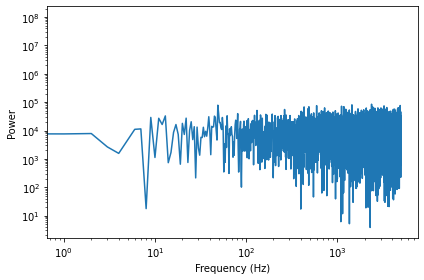
\includegraphics[width=0.8\linewidth]{resources/Images/task4_large_spectrum_log}
        \caption{Логарифмический спектр сигнала (\texttt{amp = 1}).}
        \label{fig:task4_large_spectrum_log}
    \end{figure}

    Как можно видеть из Рис.\ref{fig:task4_large_spectrum_log}, спектр этого сигнала тоже напоминает спектр белого
    шума. Оценим его наклон.

    \begin{lstlisting}[caption= Вычисление наклона \texttt{(amp = 1)}., label={lst:task4_large_slope}]
poisson_spectrum.estimate_slope().slope \end{lstlisting}

    Было получено значение 0.019870408290482002, что близко 0. А это, как уже говорилось ранее, характерно для белого шума.

    В ходе выполнения данного упражнения сначала был написан требуемый класс \texttt{UncorrelatedPoissonNoise}, генерирующий
    некоррелированный шум Пуассона. С помощью этого класса были созданы два сигнала с разной амплитудой, были получены
    их \texttt{wave} и спектры, а также оценён наклон. После этих действий был сделан вывод, что полученные сигналы
    можно отнести к белому шуму.

    \newpage

% ---------------------------------------------- Упражнение 4.5 ----------------------------------------------
    \section{Упражнение 4.5}
    \label{sec:task5}

    В этом упражнении необходимо реализовать алгоритм \texttt{Voss-McCartney} для генерации розового шума.
    Затем с помощью этого алгоритма нужно сгенерировать сигнал и убедиться, что соотношение между его мощностью
    и частотой соответствуют розовому шуму.

    Основная идея алгоритма \texttt{Voss-McCartney} заключается в сложении нескольких последовательностей случайных
    чисел, которые обновляются с разной частотой. Первый источник обновляется на каждом шаге, второй - каждый второй шаг,
    третий - каждый третий и так далее.

    Напишем метод \texttt{voss\_mccartney}, реализующий алгоритм \texttt{Voss-McCartney}.

    \begin{lstlisting}[caption= Метод \texttt{voss\_mccartney}., label={lst:task5_voss_mccartney}]
def voss_mccartney(nrows, ncols=16):
    array = numpy.empty((nrows, ncols))
    array.fill(numpy.nan)
    array[0, :] = numpy.random.random(ncols)
    array[:, 0] = numpy.random.random(nrows)

    n = nrows
    cols = numpy.random.geometric(0.5, n)
    cols[cols >= ncols] = 0
    rows = numpy.random.randint(nrows, size=n)
    array[rows, cols] = numpy.random.random(n)

    df = pandas.DataFrame(array)
    df.fillna(method='ffill', axis=0, inplace=True)
    total = df.sum(axis=1)

    return total.values \end{lstlisting}

    Теперь проверим корректную работу метода. Для этого сгенерируем 15000 значений с помощью этого метода и, используя
    их в качестве значений сигнала, преобразуем их в \texttt{wave}.

    \begin{lstlisting}[caption= Генерация значений и их преобразование в \texttt{wave}., label={lst:task5_voss_mccartney}]
ys = voss_mccartney(15000)
voss_wave = Wave(ys)
voss_wave.unbias()
voss_wave.normalize()
voss_wave.plot()
voss_wave.make_audio()  \end{lstlisting}

    \begin{figure}[H]
        \centering
        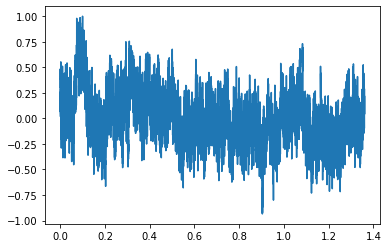
\includegraphics[width=0.75\linewidth]{resources/Images/task5_voss_wave}
        \caption{\texttt{Wave}, полученный из сгенерированных значений.}
        \label{fig:task5_voss_wave}
    \end{figure}

    Звук же сгенерированного сигнала действительно похож на шум. Теперь получим спектр мощности и заодно вычислим наклон.

    \begin{lstlisting}[caption= Вычисление логарифмического спектра., label={lst:task5_voss_spectrum}]
voss_spectrum = voss_wave.make_spectrum()
voss_spectrum.hs[0] = 0
voss_spectrum.plot()
decorate(ylabel='Power', xlabel='Frequency (Hz)', xscale='log', yscale='log')
voss_spectrum.estimate_slope().slope    \end{lstlisting}

    \begin{figure}[H]
        \centering
        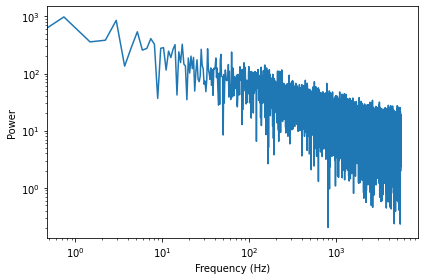
\includegraphics[width=0.75\linewidth]{resources/Images/task5_voss_spectrum}
        \caption{\texttt{Wave}, полученный из сгенерированных значений.}
        \label{fig:task5_voss_spectrum}
    \end{figure}

    Полученный спектр (Рис.\ref{fig:task5_voss_spectrum}) действительно похож на спектр розового шума. Значение наклона
    же получилось -1.0064492830615028, что можно округлить до -1. А это как раз соответствует розовому шуму.

    В ходе данного упражнения был написан метод \texttt{voss\_mccartney}, генерирующий заданное количество значений по
    алгоритму \texttt{Voss-McCartney}. Затем эти значения были преобразованы в \texttt{wave}, у которого был получен
    спектр мощности. Также был рассчитан наклон. В соответствии с полученными результатами был сделан вывод, что
    написанный метод работает корректно и подходит для генерации розового шума.

    \newpage

% ---------------------------------------------- Упражнение 3.6 ----------------------------------------------
    \section{Выводы}
    \label{sec:conclusions}

    В ходе выполнения данного лабораторной работы были изучены различные виды шумов: белый, красный и розовый.
    Кроме того, были изучены линейные и логарифмические спектры мощности. Также была проведена работа с шумами,
    имеющими природный источник. Был написан метод Бартлетта для оценки спектра мощности шумового сигнала, класс
    \texttt{UncorrelatedPoissonNoise} для генерации некоррелированного шума Пуассона и реализован алгоритм
    \texttt{Voss-McCartney} для генерации розового шума.
\end{document}